\documentclass[11pt,a4paper,titlepage]{article}

\usepackage{pdflscape}
\usepackage[margin=1in]{geometry}
\usepackage{titling}
\usepackage{graphicx}
\usepackage{titlesec}
\usepackage[hidelinks]{hyperref} 

\graphicspath{ {./Images/} }

\setcounter{secnumdepth}{4}

\titleformat{\paragraph}
{\normalfont\normalsize\bfseries}{\theparagraph}{1em}{}
\titlespacing*{\paragraph}
{0pt}{3.25ex plus 1ex minus .2ex}{1.5ex plus .2ex}

\begin{document}
%\title{ \huge Functional Requirements for the SAMBUG}

\begin{titlepage}
	
	
	\begin{center}
		\vspace*{-3cm}
  		\makebox[\textwidth]{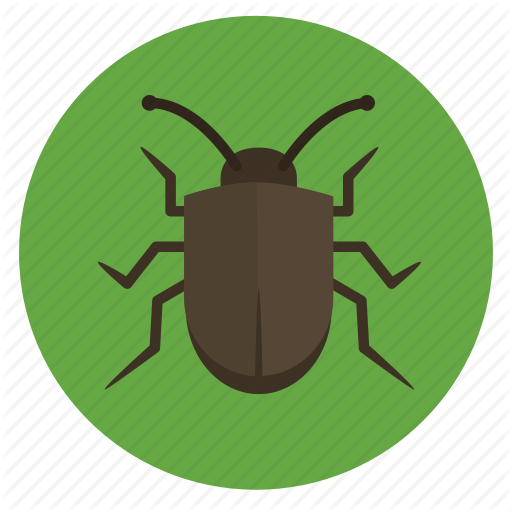
\includegraphics[width=\paperwidth]{sambug}}
	\end{center}
	
	%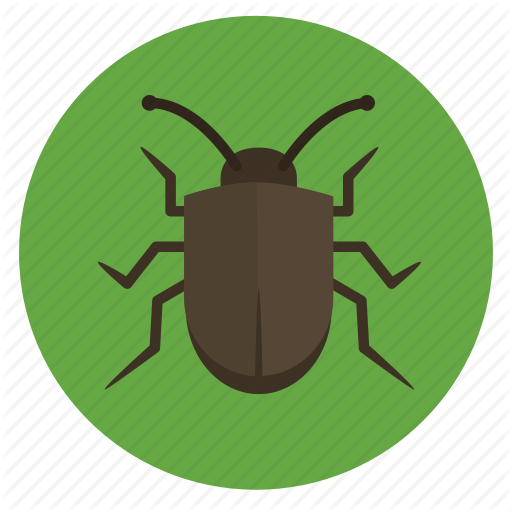
\includegraphics[width=\paperwidth]{sambug}
	
    \vspace*{2cm}
      \Huge \textbf {SAMBUG}\\
      
    \vspace*{-0.5cm}
	  \huge \textbf {User Manual}\\
	  
	\vspace*{-0.5cm}  
      \LARGE \textbf {Subtrop}
         
    \vskip2cm
          
    
    \large \textbf{July, 2015}
    \vfill
\end{titlepage}
	
	

\tableofcontents

\pagebreak

\section{System Overview}
\subsection{Introduction}
SAMBUG is a system that will ease the process of stinkbug pest scouting on a farm. Features of the system include stinkbug classification and recognition, data storage, reporting on various scouting trips and more.
\subsection{Utilisation}
Farmers can use the system in two ways, namely an Android application and a browser interface.\\\\
The way in which the system will help farmers will be listed below:
	\begin{itemize}
		\item Farmers can easily use the Android application to classify stink bugs (during a scouting trip). Classification can be done using two methods, manual classification and automatic classification:
		\begin{itemize}
			\item \textbf{Manual Classification:} This method allows the user to take a photo of a single bug and compare it with various other photos taken from a pre-selected gallery of photos. The user will select the photo that most resembles the bug that he/she wants to classify.
			\item \textbf{Automatic Classification:} This method also allows the user to take a photo of the specific bug, and thereafter the application will do the classification by using an artificially intelligent system. 
		\end{itemize}
		\item While scouting and classifying bugs, the application makes it easy to enter additional data, such as the number of that specific bug that was found, in which block of the farm it was, etc.
		\item After doing a scout trip, a summary will be shown, summarising the number and types of bugs found during that trip. Using this summary, farmers can decide with more confidence if spraying pesticide is necessary or not.
		\item When taking a photo during classification, the geolocation will be taken as well. With this feature, farmers will find it easier to make sure that scouts actually go out to random locations.
		\item After capturing the data for a scout trip, this data will be stored in a database such as to later look back at the data.
		\item The browser interface will offer various services, of which the most important is reporting services based on previous scouting trips.
		\item Administrators at Subtrop will be able to view data from different farms to also help them reach conclusions.
	\end{itemize}
	
\subsection{Intended Audience}
The intended audience of this systems is farmers specifically dealing with stink bugs as pests on their farms. Any farmer who seeks assistance with regards to bug classification, data management and scout trip management will find the system useful. The system will specifically assist farmers who do scouting of pests to reach certain conclusions, such as whether to spray pesticide or not, where and when pests are more, etc.

\subsection{Users}
The system has in mind three different users which will be described bellow:
	\begin{itemize}
		\item \textbf{Staff of Subtrop} These users will have access to all data from all the farms using the system. This means that when they log on in the browser interface they will be able to generate reports based on collective data from all farms.
		\item \textbf{Farmers} Farmers will use the browser interface, but may also use the Android application. Farmers will only be able to generate reports based on data from their own farm, thus other farms' data will not be visible. 
		\item \textbf{Scouts} Scouts will mainly use the Android Application to enter data and do classifications while in the field. The Android application is developed to keep in mind different language preferences, thus minimum usage of actual words and more symbols to carry over a message.
	\end{itemize}



\section{System Configuration}

\section{Installation}
		
\section{Getting started}

\section{Using the system}

\section{Troubleshooting}

\end{document}

%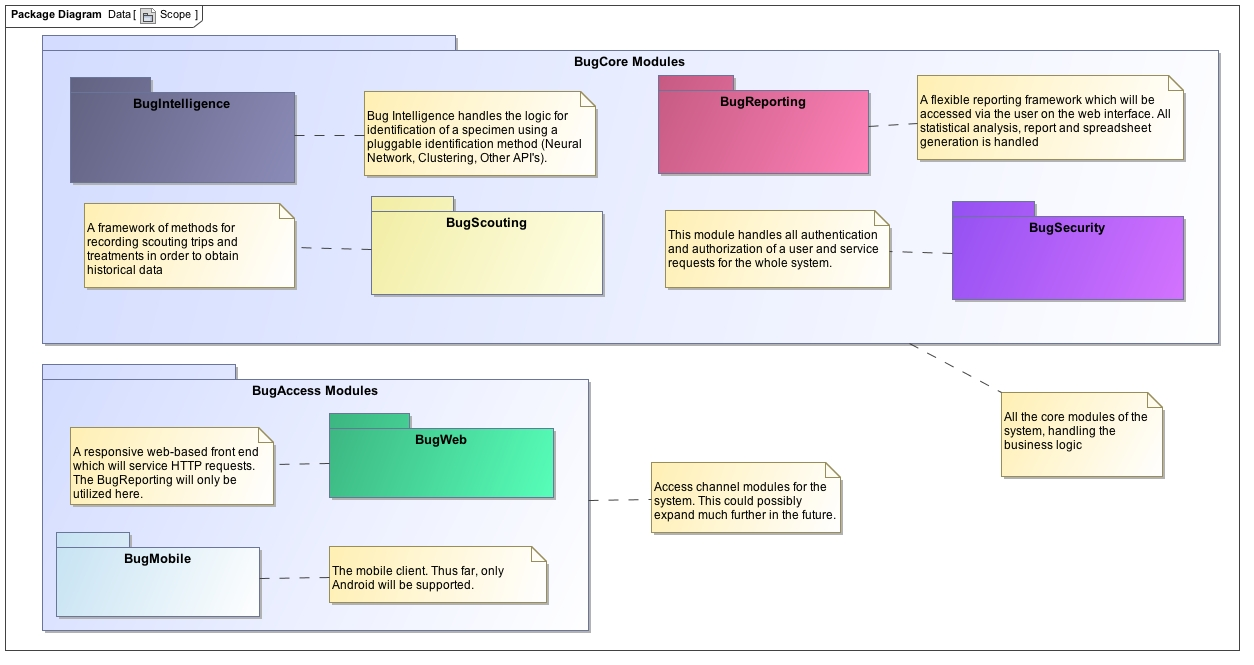
\includegraphics[width=\linewidth]{scope}